\documentclass[amsmath,amssymb,aps,prd,10pt,twocolumn,showkeys]{revtex4}
\usepackage{graphicx}
\usepackage{mathtools}
\usepackage{verbatim}
\DeclareMathOperator\erfc{erfc}
\DeclareMathOperator\erf{erf}
\DeclareMathOperator{\sgn}{sgn}
\begin{document}

\title{Complex Analysis of Askaryan Radiation: Towards UHE-$\nu$ energy Reconstruction via the Hilbert Envelope of Observed Signals}

\author{Jordan C. Hanson}
\email{jhanson2@whittier.edu}
\affiliation{Department of Physics and Astronomy, Whittier College}
\author{Raymond Hartig}
\affiliation{Department of Physics and Astronomy, Whittier College}
\date{\today}

\begin{abstract}
This is a work in progress.
\end{abstract}

\keywords{Ultra-high energy neutrino; Askaryan radiation; Mathematical physics}

\maketitle

\section{Introduction}

The introduction.

\section{Units, Definitions, and Conventions}
\label{sec:unit}

The units.

\section{Collection of Main Results}
\label{sec:onc}

Here is a list of the basic results and ideas for this paper.

\begin{itemize}
\item Let the signal model $s(t)$ be
\begin{equation}
s(t) = -E_0 t e^{-\frac{1}{2}\left(t/\sigma_t\right)^2} \label{eq:s}
\end{equation}
This is the off-cone field equation from \cite{PhysRevD.105.123019}.  The parameter $\sigma_{\rm t}$ is the pulse width, and it depends two quantities: the longitudinal length of the UHE-$\nu$-induced cascade, and the angle at which the cascade is observed relative to the Cherenkov angle.  The parameter $E_0$ is the amplitude normalization, and it depends on two parameters: $\sigma_{\rm t}$, and $\omega_{\rm 0}$, the cutoff frequency from the cascade form factor.
\item Let $\widehat{s}(t)$ represent the Hilbert transform of $s(t)$.  The \textit{analytic signal} of $s(t)$ is
\begin{equation}
s_{\rm a}(t) = s(t) + j \widehat{s}(t)
\end{equation}
The magnitude of the analytic signal, $|s_a(t)|$, is the \textit{envelope} of the signal.  The Hilbert transform $\widehat{s}(t)$ is equivalent to the convolution of $s(t)$ and the tempered distribution $h(t) = 1/(\pi t)$.
\item Let $S(f)$ be the Fourier transform of $s(t)$.  The Fourier transform of the analytic signal is
\begin{equation}
\mathcal{F}\lbrace s_{\rm a}(t) \rbrace_{f} = S_{\rm a}(f) = S(f)(1+\sgn{f}) \label{eq:sa_1}
\end{equation}
The sign function, $\sgn$ gives $-1$ if $f<0$, $0$ if $f=0$, and $1$ if $f>1$.
\item Taking the inverse Fourier transform of Eq. \ref{eq:sa_1}, the analytic signal may be written in terms of $S(f)$:
\begin{equation}
s_{\rm a}(t) = 2\int_{0}^{\infty} S(f) e^{2\pi j f t} df \label{eq:sa_2}
\end{equation}
\item The Fourier transform of Eq. \ref{eq:s} is
\begin{equation}
S(f) = E_0 \sigma_t^3 (2\pi)^{3/2} j f e^{-2\pi^2 f^2 \sigma_t^2}
\end{equation}
\item Using the gaussian spectral width $\sigma_{\rm f}$ from \cite{10.1016/j.astropartphys.2017.03.008}, and the guassian width of $s(t)$ from \cite{PhysRevD.105.123019}, it was shown in \cite{PhysRevD.105.123019} that the uncertainty principle holds for off-cone signals:
\begin{equation}
\sigma_t \sigma_f \geq \frac{1}{2\pi}
\end{equation}
The equality is reached in the limit the far-field parameter limits to zero: $\eta \to 0$.  This makes the signal spectrum
\begin{equation}
S(f) = E_0 \sigma_t^3 (2\pi)^{3/2} j f e^{-\frac{1}{2}\left(f/\sigma_f\right)^2} \label{eq:spec}
\end{equation}
Inserting $S(f)$ into Eq. \ref{eq:sa_2}, $s_{\rm a}(t)$ is
\begin{equation}
s_{\rm a}(t) = \frac{E_0 \sigma_t^3 (2\pi)^{3/2}}{\pi} \frac{d}{dt}\int_0^{\infty} e^{-\frac{1}{2}\left(f/\sigma_f\right)^2} e^{2\pi j f t} df \label{eq:sa_3}
\end{equation}
\item Let $k^2/4 = \frac{1}{2}\left(f/\sigma_f\right)^2$, and $x = t/(\sqrt{2}\sigma_t)$.  Equation \ref{eq:sa_3} can be broken into real and imaginary parts:
\begin{align}
s_{\rm a}(t) &= \frac{E_0 \sigma_{\rm t}}{\sqrt{2\pi}}\frac{dI}{dx} \\
\Re\lbrace I \rbrace &= \int_0^{\infty} e^{-k^2/4}\cos(kx) dk \\
\Im\lbrace I \rbrace &= \int_0^{\infty} e^{-k^2/4}\sin(kx) dk
\end{align}
The real part of $I$ is even, so it can be extended to $(-\infty,\infty)$ if it is multiplied by $1/2$.  The result is
\begin{equation}
\Re\lbrace I \rbrace = \sqrt{\pi} e^{-x^2}
\end{equation}
The imaginary part of $I$ is proportional to \textit{Dawson's integral, $D(x)$} \cite{NIST:DLMF}:
\begin{equation}
\Im\lbrace I\rbrace = 2 D(x)
\end{equation}
\item The overall analytic signal, $s_a(t)$, is
\begin{equation}
s_a(t) = -E_0 \left(t e^{-\frac{1}{2}\left(t/\sigma_t\right)^2} - \frac{2 j\sigma_t}{\sqrt{2\pi}} \frac{dD(x)}{dx}\right) \label{eq:sa_4}
\end{equation}
The signal envelope is $|s_a(t)|$.  It is important to note that, though $D(x)$ is not evaluated analytically, a high-precision algorithm for computing $D(x)$ was given in \cite{10.1063/1.4822832}.  Note that $s_a(0) \neq 0$, since $dD(x)/dx = 1 - 2x D(x)$.
\item Signal data in detectors designed to observe Askaryan pulses is equivalent to the convolution of the signal and detector response functions.  Signal models are convolved with measured detector responses to create \textit{signal templates}.  Signal templates are cross-correlated with observed data to identify UHE-$\nu$ signals.  The oscillations of signal templates and observed data can introduce various uncertainties when cross-correlated.  This problem intensifies when the signal-to-noise ratio between Askaryan pulse data and thermal noise decreases.  To reduce these uncertainties, the Hilbert envelope of observed signals is used in cross-correlations instead of the original signals.  We seek an analytic equation for the Hilbert envelope of the data.  That is, we seek the envelope of the convolution of the analytic signal model with a typical detector response.  The RLC damped oscillator is a standard circuit model for the RF dipole antennas used in RNO-G and the proposed IceCube Gen2 \cite{10.1103/PhysRevD.85.062004,10.1088/1748-0221/16/03/p03025,10.48550/arxiv.2008.04323}.
\item There are two paths to calculating the final result.  The first option involves three steps.  First, the detector response, $r(t)$ is convolved with $s(t)$.  Second, the analytic signal of the result is found.  Third, the magnitude of the analytic signal is computed, which can be compared to envelopes of observed signals.  The second option involves computing the envelope of the convolution of $r(t)$ with $s(t)$ directly from $s_a(t)$ and $r_a(t)$.
\item Let $s(t) * r(t)$ represent the convolution of $s(t)$ and $r(t)$.  Let the envelope of the convolution be $\mathcal{E}_{s * r}(t)$.  $\mathcal{E}_{s * r}(t)$, $s_a(t)$, and $r_a(t)$ are related by
\begin{equation}
\mathcal{E}_{s * r}(t) = \frac{1}{2}| s_a (t) * r_a(t)| \label{eq:awesome}
\end{equation}
The proof of Eq. \ref{eq:awesome} is based on two ideas.  First, the Hilbert transform of a function $s(t)$ is equivalent to convolving it with the ``tempered distribution'' $h(t) = 1/(\pi t)$.  Second, computing the Hilbert transform twice yields the original function, multiplied by $-1$: $h * h * s = -s$.  Given the definitions of the analytic signal and the Hilbert transform,
\begin{align}
(s * r)_a (t) &= s * r + j ~ \widehat{s*r} \\
\mathcal{E}_{s * r}(t) &= | s * r + j s * r * h|
\end{align}
However,
\begin{align}
r_a * s_a &= (r + j \hat{r}) * (s + j \hat{s}) \\
r_a * s_a &= r * s + j r * \hat{s} + j \hat{r} * s - \hat{r} * \hat{s} \\
r_a * s_a &= r * s - r * h * s * h + 2 j h * r * s \\
r_a * s_a &= r * s - h * h * r * s + 2 j h * r * s \\
r_a * s_a &= 2 r * s + 2 j h * r * s
\end{align}
Multiplying both sides $1/2$ and taking the magnitude completes the proof:
\begin{equation}
\frac{1}{2} |r_a * s_a| = |r * s + j h * r * s| = \mathcal{E}_{s * r}(t) \\
\end{equation}
\item Assume that a signal arrives in an RLC damped oscillator at $t=0$.  For $t\geq 0$, the impulse response and corresponding analytic signal are
\begin{align}
r(t) &= R_0 e^{-2 \pi \gamma_f t} \cos(2\pi f_0 t) \label{eq:r} \\
r_a(t) &= R_0 e^{-2 \pi \gamma_f t} e^{2\pi j f_0 t} \label{eq:ra}
\end{align}
The parameters $\gamma_f$ and $f_0$ are the \textit{decay constant} that corresponds to the \textit{fall time} of the output signal, and the resonance frequency.  Note that the envelope of $r(t)$, $|r_a(t)|$, is $R_0 \exp(-2 \pi \gamma_f t)$, as expected.  To prove Eq. \ref{eq:ra}, first compute the Fourier transform of $r(t)$:
\begin{align}
R(f) &= \frac{R_0}{4\pi j} \left( \frac{1}{f - z_{+}} + \frac{1}{1- z_{-}} \right) \\
z_{+} &= f_0 + j \gamma_f \\
z_{-} &= -f_0 + j \gamma_f
\end{align}
Given Eq. \ref{eq:sa_2}, the procedure to find $r_a(t)$ is to multiply the \textit{negative} frequency components by 0 and the \textit{positive} frequency components by 2, and take the inverse Fourier transform.  The inverse Fourier transform may be completed by extension to the complex plane using the upper infinite semi-circle as a contour, and applying Jordan's lemma.  The residue from the pole at $z_{+}$ drives the final result.
\item The goal is now to apply Eq. \ref{eq:awesome} by convolving $s_a(t)$ with $r_a(t)$.  The calculation may be split into two parts: $r_a(t) * \Re\lbrace s_a(t) \rbrace$, and $r_a(t) * \Im\lbrace s_a(t) \rbrace$.  Let $u(t)$ represent the Heaviside step function.  Starting with $r_a(t) * \Re\lbrace s_a(t) \rbrace$:
\begin{multline}
r_a(t) * \Re\lbrace s_a(t) \rbrace = \\ R_0 e^{2\pi j f_0 t} e^{-2\pi\gamma t} u(t) * \left(-E_0 t e^{-\frac{1}{2}\left(t/\sigma_t\right)^2}\right)
\end{multline}
Let $x=t/(\sqrt{2}\sigma_t)$, $y=\tau/(\sqrt{2}\sigma_t)$, and $z = (2\pi j f_0 - 2\pi\gamma)\sqrt{2}\sigma_t$.  Changing variables while accounting for the relationship between $u(t)$, $x$, and $y$, gives
\begin{multline}
r_a(t) * \Re\lbrace s_a(t) \rbrace = \\ -2R_0 E_0 \sigma_t^2 \int_{-\infty}^{x} e^{z(x-y)} y e^{-y^2} dy
\end{multline}
Note that the units for the convolution of $r(t)$ and $s(t)$ correspond to $R_0 E_0 \sigma_t^2$.  Let $u = x-y$, so that $du = -dy$. The result is
\begin{equation}
r_a(t) * \Re\lbrace s_a(t) \rbrace = 2R_0 E_0 \sigma_t^2\left(\frac{dI(x,z)}{dz}-xI(x,z)\right)
\end{equation}
where
\begin{equation}
I(x,z) = \int_0^{\infty} e^{zu} e^{-(u-x)^2} du
\end{equation}
Let $b = x+\frac{1}{2} z$. Completing the square in the exponent and substituting $k = u-b$ gives
\begin{multline}
I(x,z) = e^{-x^2} e^{b^2} \int_{-b}^{\infty} e^{-k^2} dk \\ = \frac{\sqrt{\pi}}{2} e^{-x^2} e^{b^2} \erfc(-b)
\end{multline}
Let $b = jq$, and $w(q)$ be the \textit{Faddeeva function} \cite{NIST:DLMF}.  The integral becomes
\begin{equation}
I(x,z) = \frac{\sqrt{\pi}}{2} e^{-x^2} w(q)
\end{equation}
The chain rule is required to find $dI/dz$:
\begin{equation}
\frac{dI}{dz} = \frac{dI}{dq}\frac{dq}{dz} = -\left(\frac{j}{2}\right)\frac{dI}{dq}
\end{equation}
The final result is
\begin{multline}
r_a(t) * \Re\lbrace s_a(t) \rbrace = \\ -\sqrt{\pi} R_0 E_0 \sigma_t^2 \left(x e^{-x^2} w(q) + \left(\frac{j}{2}\right) e^{-x^2} \frac{dw(q)}{dq} \right) \label{eq:Re_result}
\end{multline}
\item Turning to the convolution of $r_a(t)$ with $\Im(s_a)$,
\begin{multline}
r_a(t) * \Im\lbrace s_a(t) \rbrace = \\ \left(R_0 e^{2\pi j f_0 t} e^{-2\pi \gamma t} u(t)\right) * \left(\frac{2 E_0 \sigma_t^2}{\sqrt{\pi}}\frac{dD(t/\sqrt{2}\sigma_t)}{dt} \right)
\end{multline}
Note that $f'(t) * g(t) = f(t) * g'(t) = (f(t) * g(t))'$.  Thus,
\begin{multline}
r_a(t) * \Im\lbrace s_a(t) \rbrace = \\ \frac{2}{\sqrt{\pi}} R_0 E_0 \sigma_t^2 \frac{d}{dt}\left(e^{2\pi j f_0 t}e^{-2\pi\gamma t} u(t) * D(t/\sqrt{2}\sigma_t) \right)
\end{multline}
Accounting for the step function in the convolution gives
\begin{multline}
r_a(t) * \Im\lbrace s_a(t) \rbrace = \\ \frac{2}{\sqrt{\pi}} R_0 E_0 \sigma_t^2 \frac{d}{dt} \int_{-\infty}^{t} e^{(2\pi j f_0 - 2\pi\gamma)(t-\tau)}D(\tau/\sqrt{2}\sigma_t)d\tau
\end{multline}
Adopting the earlier definitions of $x$, $y$, and $z$ gives
\begin{multline}
r_a(t) * \Im\lbrace s_a(t) \rbrace = \\ \frac{2}{\sqrt{\pi}} R_0 E_0 \sigma_t^2 \frac{d}{dx} \int_{-\infty}^{x} e^{z(x-y)} D(y) dy
\end{multline}
Using the fundamental theorem of calculus, and the limiting cases of $D(x)$, 
\begin{multline}
r_a(t) * \Im\lbrace s_a(t) \rbrace = \\ \frac{2}{\sqrt{\pi}} R_0 E_0 \sigma_t^2 \left(D(x) + z\int_{-\infty}^{x} e^{z(x-y)} D(y) dy \right)
\end{multline}
Let $u = x-y$, $z=-k$, and note that $D(x)$ is an odd function.  These substitutions give
\begin{multline}
r_a(t) * \Im\lbrace s_a(t) \rbrace = \\ \frac{2}{\sqrt{\pi}} R_0 E_0 \sigma_t^2 \left(D(x) + k\int_{0}^{\infty} e^{-ku} D(u-x) du \right)
\end{multline}
The remaining integral is the Laplace transform of the shifted Dawson function, $\mathcal{L}\lbrace D(u-x)\rbrace_k$.  The final result is
\begin{equation}
r_a(t) * \Im\lbrace s_a(t) \rbrace = \\ \frac{2}{\sqrt{\pi}} R_0 E_0 \sigma_t^2 \left(D(x) + k\mathcal{L}\lbrace D(u-x)\rbrace_k\right) \label{eq:Im_result}
\end{equation}
Though a closed analytic form for $\mathcal{L}\lbrace D(u-x)\rbrace_k$ is elusive, finishing this calculation through numerical integration is straightforward.
\item Combining Eq. \ref{eq:Re_result} and Eq. \ref{eq:Im_result} gives $r_a(t) * s_a(t)$, since
\begin{equation}
r_a(t) * s_a(t) = r_a(t) * \Re\lbrace s_a(t)\rbrace + j r_a(t) * \Im\lbrace s_a(t)\rbrace
\end{equation}
which yields
\begin{multline}
r_a(t) * s_a(t) = \\ -\sqrt{\pi} R_0 E_0 \sigma_t^2 \left(x e^{-x^2} w(q) + \left(\frac{j}{2}\right) e^{-x^2} \frac{dw(q)}{dq} \right) + \\ \frac{2j}{\sqrt{\pi}} R_0 E_0 \sigma_t^2 \left(D(x) + k\mathcal{L}\lbrace D(u-x)\rbrace_k\right) \label{eq:final}
\end{multline}
The units of convolution should be $R_0 E_0\sigma_t^2$, and each term in Eq. \ref{eq:final} has these units.  Remember that the relationship between $q$ and $x$ is given by
\begin{equation}
q = -jb = -j\left(x + \frac{z}{2}\right) \\
\end{equation}
Taking the magnitude of Eq. \ref{eq:final}, and multiplying by $1/2$, yields the \textbf{Hilbert envelope of the convolution of $s(t)$ with $r(t)$:}
\begin{equation}
\mathcal{E}_{r * s}(t) = \frac{1}{2} | r_a(t) * s_a(t) | \label{eq:final2}
\end{equation}
\item It is important to note that the convolution of $s(t)$ and $r(t)$ may be done analytically in the time-domain:
\begin{equation}
s * r = \int_{-\infty}^{\infty} s(t-\tau) r(\tau) d\tau 
\end{equation}
Inserting the definitions of $s(t)$ and $r(t)$,
\begin{multline}
s * r = \\ -E_0 R_0 \int_{-\infty}^{\infty} (t-\tau) e^{-\frac{1}{2}\left(\frac{t-\tau}{\sigma_t}\right)^2} \Re\left\lbrace e^{2\pi j f_0 \tau} e^{-2\pi\gamma \tau} \right\rbrace u(\tau) d\tau
\end{multline}
Using the previous definitions of $x$, $y$, and $z$ gives
\begin{equation}
s * r = -2R_0 E_0 \sigma_t^2 \int_{0}^{\infty} (x-y) e^{-(x-y)^2} \Re\left\lbrace e^{zy} \right\rbrace dy
\end{equation}
Note that the $\Re\lbrace \rbrace$ operator can encompass the whole integral, since $s(t)$ is real.  Splitting the integral and employing differentiation under the equals sign yields
\begin{multline}
s * r = \\ -2R_0 E_0 \sigma_t^2 \Re\left\lbrace xe^{-x^2}I(x,z) - \frac{1}{2}e^{-x^2} \frac{dI(x,z)}{dx} \right\rbrace \label{eq:conv_sr}
\end{multline}
with
\begin{equation}
I(x,z) = \int_0^{\infty} e^{-y^2 + (2x + z)y}dy
\end{equation}
As above, let $b=x+\frac{1}{2}z$, and $b = j q$.  In a procedure resembling the calculation for $r_a(t) * \Re\lbrace s_a(t)\rbrace$, the result for $I(x,z)$ is
\begin{equation}
I(x,z) = \frac{\sqrt{\pi}}{2} w(q)
\end{equation}
where $w(q)$ is the Faddeeva function.  Note that the Faddeeva function is \textit{entire}, meaning the $\Re\lbrace \rbrace$ operator and differentiation commute.  Inserting this result into Eq. \ref{eq:conv_sr}, and distributing the $\Re\lbrace \rbrace$ operator to the instances of $I(x,z)$, gives
\begin{multline}
s * r = -\sqrt{\pi}R_0 E_0 \sigma_t^2 \\ \left(xe^{-x^2} \Re\left\lbrace w(q)\right\rbrace - \frac{1}{2}e^{-x^2} \frac{d\Re\lbrace w(q)\rbrace}{dx} \right)
\end{multline}
From the definition of $q$ and the chain rule, $dw(q)/dx = -jdw(q)/dq$, and $dw(q)/dq = -2qw(q)+2j/\sqrt{\pi}$ \cite{NIST:DLMF}.  The final result is left in terms of the real part of the Faddeeva function, which may be computed using the \textit{Voigt function} $U(x,t)$ \cite{NIST:DLMF,PhysRevD.105.123019}.
\begin{multline}
s * r = -\sqrt{\pi}R_0 E_0 \sigma_t^2 \\ \left(xe^{-x^2} \Re\left\lbrace w(q)\right\rbrace + j\frac{1}{2}e^{-x^2} \frac{d\Re\lbrace w(q)\rbrace}{dq} \right) \label{eq:final3}
\end{multline}
\item To illustrate the accuracy and efficiency of the model, Eq. \ref{eq:final}-\ref{eq:final2} and \ref{eq:final3}, are shown in Fig. \ref{fig:fig1}.
\begin{figure}
\centering
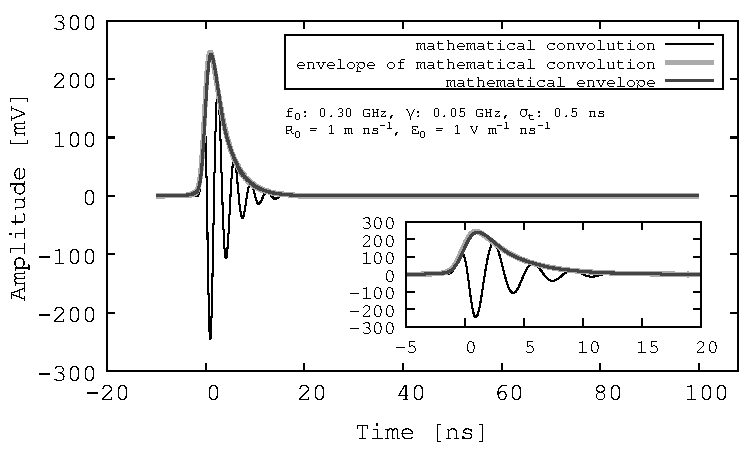
\includegraphics[width=0.5\textwidth]{July3rd_plot1.pdf}
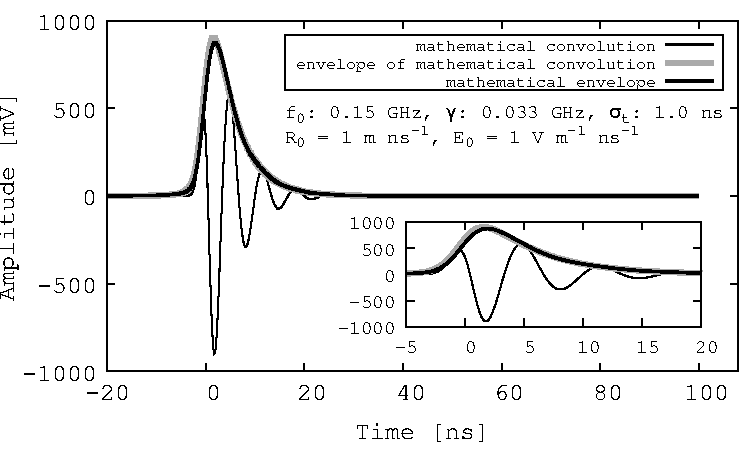
\includegraphics[width=0.5\textwidth]{July3rd_plot2.pdf}
\caption{\label{fig:fig1} (Top) The thin black line represents $s(t) * r(t)$.  The light gray envelope represents the envelope of $s(t) * r(t)$ computed with the Python3 SciPy function scipy.special.hilbert. The dark gray envelope represents Eq. \ref{eq:final}-\ref{eq:final2}. (Bottom) Same as top, for different parameter values.}
\end{figure}
\item To demonstrate that \textit{numerical convolution} of $s(t)$ and $r(t)$ produces the same results as the \textit{mathematical convolution} of $s(t)$ and $r(t)$ (Eq. \ref{eq:final3}), the corresponding waveforms are shown in Fig. \ref{fig:fig2}.
\begin{figure}
\centering
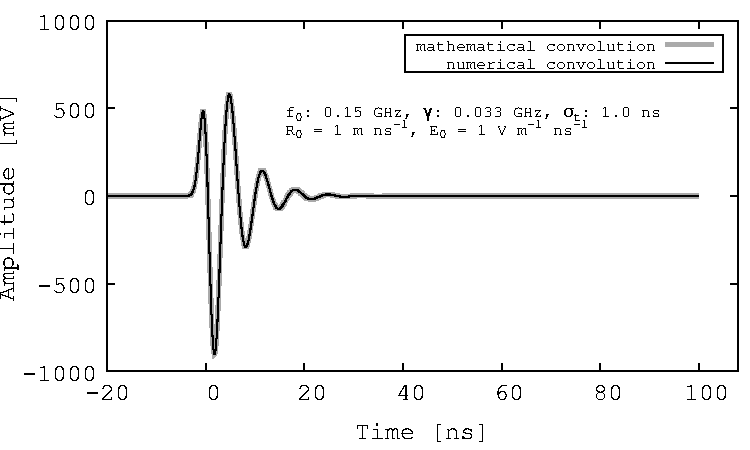
\includegraphics[width=0.5\textwidth]{July7th_plot1.pdf}
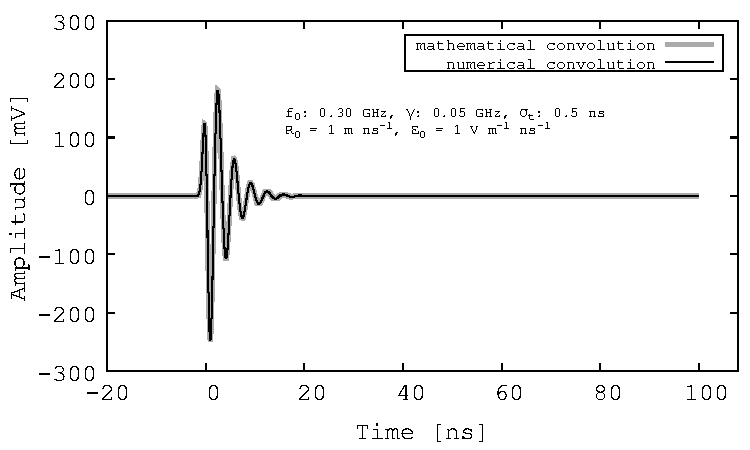
\includegraphics[width=0.5\textwidth]{July7th_plot2.pdf}
\caption{\label{fig:fig2} (Top) The thin black line represents $s(t) * r(t)$, produced using the Python3 SciPy function scipy.signal.convolve. The dark gray line represents Eq. \ref{eq:final3}. (Bottom) Same as top, for different parameter values.}
\end{figure}
\end{itemize}

\section{Conclusion}
\label{sec:conc}

The conclusion.

\appendix

\section{Details}
\label{app:a}

The details.

\bibliography{apssamp}

\end{document}

